\chapter{Algoritmo ottimizzato tramite decomposizioni bilanciate}
\label{cap:3}
In questo capitolo viene presentata un'ottimizzazione all'algoritmo descritto nel capitolo \ref{cap 2}. 
basata sull'idea di decomporre gli alberi $T$ in una coppia di alberi $T'$ e $T''$ con un numero simile di nodi.
Si fa vedere, inoltre, come modificare i dettagli implementativi precedentemente discussi.

\section{Decomposizioni bilanciate di un albero}
\label{cap:3 par:1}
Nel precedente capitolo, dato un albero $ T $ con $|T|=k$, viene considerata la decomposizione di $T$ in due alberi $ T' $ e $ T''$. 
Dipendentemente da $T$, tale decomposizione può restituire un albero $T'$ (o $T''$) contenente un numero esiguo di nodi rispetto a $|T|$.
Un esempio dove questo fenomeno è particolarmente evidente si verifica quando $T$ è una stella di $k$ nodi per cui $|T'|=k-1$ e $|T''|=1$.

In questa sezione si mostrerà che dato un albero $T$ \`e sempre possibile ricavare una decomposizione ``bilanciata'' dell'albero  in due alberi $ T' $ e $ T'' $ le cui cardinalit\`a distino al al più di una costante moltiplicativa.

Prima di poter enunciare e dimostrare il risultato principale occorre dare delle nozioni preliminari.

\newtheorem{definizione}{Definizione}[section]

\begin{definizione}
	\label{definizioneDeco} 
Sia $T_r$ un albero, con $k$ nodi, radicato nel nodo $r$.
Diremo che la coppia $(A,B)$, dove  $A$ e $B$ sono due sottoalberi di $T_r$, \`e una decomposizione per l'albero $ T_r $ se:
\begin{itemize}
	\item $| A | + | B | = k$; e
\item $A \ e \  B $ condividono solo il nodo $ r $.
\end{itemize}
\end{definizione}


\begin{definizione}
\label{lemmaDeco}
Data una funzione $f : \mathbb{N} \to \mathbb{N}$ ed un albero $ T $ con $ k $, diremo che $ (A,B) $ \`e una decomposizione $ f(k) $-bilanciata se:
\begin{equation*}
	\max{ \{|A| , |B| \} }  \le  f(k).
\end{equation*}
\end{definizione}


Una nozione che sarà utile nel seguito è quella di $ centroide $ di un albero, definito come segue:

\begin{definizione}
Per ogni nodo $ v $ di un albero $ T $, le diramazioni di $ T $  rispetto a $ v $, sono tutti i sottoalberi massimali di $ T $ non contenenti $ v $. 
Per ogni $ v \in T $, si definisce $\alpha(v)$ come il massimo numero di nodi tra le diramazioni rispetto a $ v $.\\ 
Un nodo $ v $ di un albero $ T $ con $ n $ nodi, \`e un nodo centroide se $\alpha(v)\le\frac{n}{2}$.
\end{definizione}

Il centroide di un albero non \`e necessariamente unico, infatti Jordan \cite{jordan1869assemblages}  ha dimostrato che, dato un albero $ T $ con $ n $ nodi:
\begin{enumerate}
	\renewcommand{\labelenumi}{\roman{enumi}}
	\item $ T $ ha un singolo centroide $ v $ e $\alpha(v) < \frac{n}{2}$, oppure
	\item$ T $ ha due nodi centroidi (adiacenti) $v_1$ e $v_2$ tali che $\alpha(v_1) = \alpha(v_2) = \frac{n}{2}$, in questo caso il numero di nodi $ n $ \`e pari.
\end{enumerate}

Esistono diversi algoritmi per la ricerca del centroide, quello utilizzato in questa tesi \`e un algoritmo con complessit\`a temporale lineare nel numero di nodi che fa uso di una visita in profondità (DFS) dell'albero. \\
Il primo passo da effettuare \`e calcolare i valori $\alpha(v)$ per ogni nodo $ v$ dell'albero $T$.\\
Innanzitutto per ogni nodo $v$ di $T $ indichiamo con $ \eta(v) $ il numero di nodi presenti nel sottoalbero radicato in $ v $ di $ T $.
A questo punto si radica $T$ in un nodo arbitrario e si procede ad una visita DFS dell'albero, memorizzando, per ogni $v$, il rispettivo valore $ \eta(v) $, che può essere calcolato ricorsivamente nel seguente modo 
\begin{equation}
\label{eq:eta_centroide}
\eta(v) = 1 + \sum_{\substack{u \ figlio \ di \ v \ in \ T} } { \eta(u)}.
\end{equation}

Si noti che, nel caso particolare in cui $v$ è una foglia, la formula precedente implica che $\eta(v)=1$.
Una volta conclusa la visita, si pu\`o determinare $ \alpha(v) $ per ogni nodo $ v $ in $ T $, come segue
\[ \alpha(v) = \max\{ \max_{\substack{u \ figlio \ di \ v \ in \ T}} {\eta(u)} \ , \ |T| - \eta(v) \}. \]
\noindent Una volta calcolato il valore di $ \alpha(v) $ per ogni $  v \in T $ si verifica per quali valori  risulta $\alpha(v)\le\frac{|T|}{2}$.\\
%Nel caso ci fosse un unico nodo $ v $ che soddisfa la precedente condizione, come in (i),  allora tale nodo rappresenta l'unico  centroide dell'albero $ T $.
%Nel caso, invece, ce ne fossero due, come in (ii), per esempio $ v_1 $ e $ v_2 $,  l'albero $ T $ conterr\`a due centroidi, rispettivamente $ v_1 $ e $ v_2 $.\\
Per verificare che l'algoritmo ha una complessit\`a $ T(n) $ lineare sul numero di nodi.
Basta notare che la visita DFS su un albero $ T $ di $ n $ nodi richiede un tempo $ O(n) $ per essere completata.

A questa quantità va sommato il tempo necessario per calcolare, per ogni nodo $v$ di $T$, la quantità $\eta(v)$ usando la formula \eqref{eq:eta_centroide}. Ciò richede tempo $O(1 + \delta(v))$ dove $\delta(v)$ indica il grado di $v$ in $T$.

In particolare insieme quanto detto finora, ed usando l'identità $\sum_{v} \delta(v) = 2(n-1)$, quello che si ottiene \`e:
\[  T(n) = O(n + \sum_{v}(1+\delta(v)))= O(n + n + \sum_{v}\delta(v)) = O(n+n+2n-2)=O(n).
\] 

Nell'esempio \ref{es1} si pu\`o vedere l'applicazione dell'algoritmo per la ricerca del centroide.
	\begin{figure}[htbp]
		\centering
		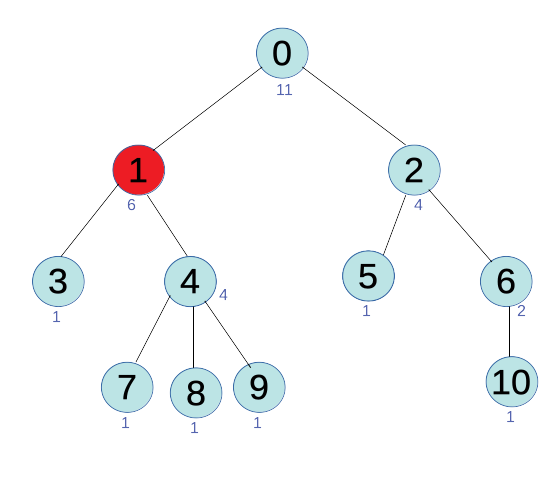
\includegraphics[width=5cm]{capitolo3/grafo2}
		\caption{Albero $ T $  per la ricerca del centroide} 
		\label{fig:2}
\end{figure}

\newtheorem{esempio}[definizione]{Esempio}
\begin{esempio}
	\label{es1}
Si consideri l'albero T in figura \ref{fig:2} per la ricerca del nodo centroide.
Per ogni nodo $ v $ di $ T $ numerato da 0 a 10,  viene calcolato $\alpha(v)$ . \\
Per prima cosa calcoliamo il valore di $ \eta(v) $ per ogni $ v $ di $ T $.
Avremo:
\begin{center} 
	\centering
	\begin{tabular}{ c c c c c}
		$ \eta(0) = 11 $ & & $ \eta(1)= 4 $ && $ \eta(2) = 6 $ \\
		$ \eta(3) = 2 $ & & $ \eta(4) = 1 $ && $ \eta(5) = 4 $ \\
		$ \eta(6) = 1 $ & & $ \eta(7) = 1 $ && $ \eta(8) = 1 $ \\
		$ \eta(9) = 1 $ & & $ \eta(10) = 1 $ \\
	\end{tabular}

	
	
\end{center}
Pertanto $ \alpha(v) $ per ogni $ v $ sarà: 
\begin{center}
	\centering
	\begin{tabular}{ c c c c c  }
		$\alpha(0) = \max\{6,0\}$ & & $\alpha(1) = \max\{2,7\}$ & & $\alpha(2) =\max\{4,5\} $ \\ 
		$\alpha(3) = \max\{1,9\}$ && $\alpha(4) =\max\{0,10\}$ &&  $\alpha(5) = \max\{1,7\}$ \\  
		$\alpha(6) = \max\{0,10\}$ && $\alpha(7) = \max\{0,10\}$ && $\alpha(8) = \max\{0,10\}$ \\
		$\alpha(9) = \max\{0,10\}$ && $\alpha(10) = \max\{0,10\}$ &&
	\end{tabular}
\end{center}

Poich\'e $ \left\lfloor\frac{n}{2} \right\rfloor = \left\lfloor \frac{11}{2} \right\rfloor = 5$, l'unico nodo per cui la disuguaglianza, $\alpha(v)\le\frac{n}{2}$, risulta vera \`e il nodo 2, infatti $5\le 5$.\\
Poich\`e il numero di nodi \`e dispari certamente questo sar\`a l'unico centroide dell'albero T (figura \ref{fig:2}). 
\demo
\end{esempio}\mbox{}\\

L'ultimo punto da considerare prima di poter enunciare e dimostrare il risultato principale di questa sezione riguarda la definizione di un algoritmo valido per decomporre un albero in due sottoalberi che chiameremo $ T' $ e $ T'' $, in maniera $ f(k) $-bilanciata.\\
Sia dato in input un albero $ T $, con $ k\ge 3 $ nodi e
si supponga, senza perdita di generalit\`a, che i sottoalberi radicati nei figli della radice $ r $ di $ T $ siano ordinati in ordine non crescente rispetto al rispettivo numero di nodi.
Da questo deriva che, supponendo che $ r $ abbia $ \ell $ figli, vi saranno $ \ell $ alberi radicati tali che: $ |T_{i}|\ge |T_{i+1}| \ \  \forall {i = 1,\dots, \ell-1} $, inoltre si indica con $ S $ la seguente quantit\`a $ S=\sum_{i=1}^{\ell}|T_i| $.
Sia $i = \max \{ j : \sum_{h=1}^{j} |T_h| \le \frac{2 S}{3} \}$. L'algoritmo selezionerà $T'$ come il sottoalbero di $T$ indotto da $r$ e dai nodi in $T_1, \dots, T_i$, e $T''$ di conseguenza.
La decomposizione di $T$ in $T'$ e $T''$ restituita dall'algoritmo appena descritto, il cui pseudocodice è mostrato nell'algoritmo \ref{algoritmo1}, è $ (\lfloor \frac{2}{3}(k-1) \rfloor + 1)$-bilanciata, come dimostrato dal teorema a seguire.

	\begin{figure}[htbp]
	\centering
	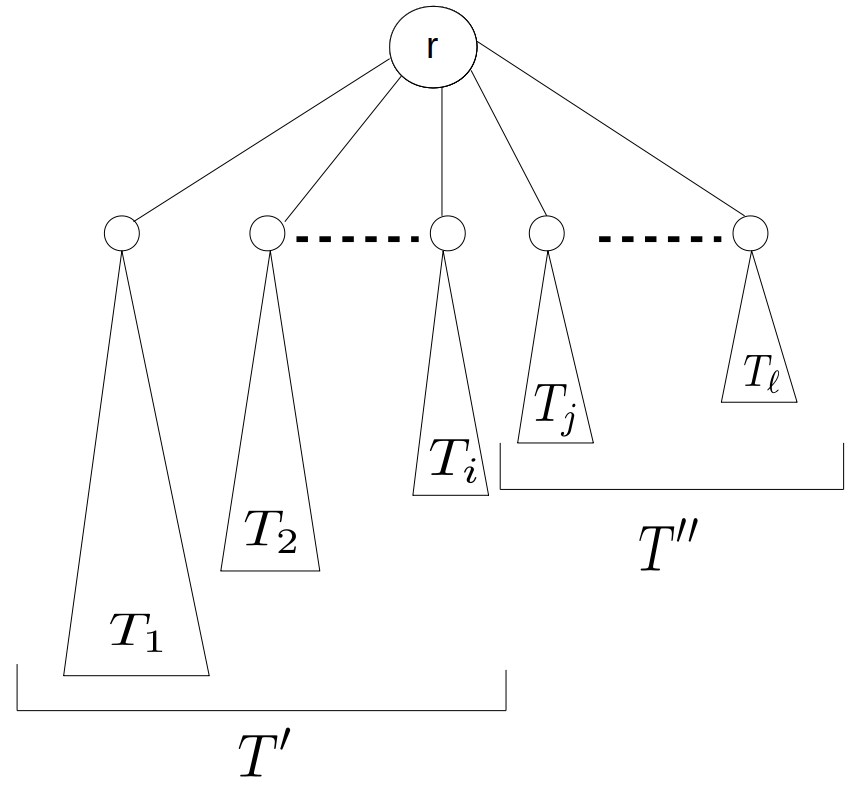
\includegraphics[width=6.5cm]{capitolo3/grafo4}
	\caption{Esempio di albero $ T $ radicato in $ r $, con $ k $ nodi, decomposto secondo l'algoritmo \ref{algoritmo1} in due alberi $ T' $ e $ T'' $.}
	\label{fig:3} 
\end{figure}

\begin{algorithm}[H]
	\label{algoritmo1}
	\SetAlgoLined
	\caption{Algoritmo per il calcolo di una decomposizione $ (\lfloor \frac{2}{3}(k-1) \rfloor + 1)$-bilanciata di un albero $T$ }
	\textbf{input} : Albero $ T $ con $ k $ nodi\;
	$r \gets $ un centroide di $T$\;
	$T_r \gets $ albero $T$ radicato in $r$\;
	$\ell \gets$ grado di $r$ in $T$\; 
	Sia $T_i$ l'albero radicato nell'$ i $-esimo figlio di $ r $ e $V_i$ l'insieme dei nodi di $T_i$ \;
	Si considerino gli alberi $T_i$ in ordine non crescrente rispetto al rispettivo numero di nodi, i.e., $ |T_{i}|\ge |T_{i+1}| \ \ \forall {i = 1,\dots, \ell-1} $\;
	
	$ S \gets \sum_{i=1}^{n}|T_i| $;\\
	\For{$ i = 1,\dots,\ell $}
	{
		\If{$ \sum_{j=1}^{i}{|T_j|} > \frac{2}{3}\cdot S $}
		{
			$ T'\gets $ sottoalbero di  di $ T_r $ indotto da $ \{r\} \cup \bigcup_{j=1}^{i-1} V_j$\; %TODO Hai definito la notazione V(T)??
			$ T'' \gets $ sottoalbero di $ T_r $ indotto da \{r\} \cup \bigcup_{j=i}^\ell V_j\;
			\textbf{return} ($ T',T'' $);\;
		}	 
}
\end{algorithm}



\newtheorem{teorema1}[definizione]{Teorema}
\begin{teorema1}
	\label{teorema1 cap3 sez1}
Per ogni albero T di $k \ge 3$ nodi esiste un nodo $r$ di T  tale che l'albero $T_r$, ottenuto radicando $T$ in $r$, ammette una decomposizione $ (\lfloor \frac{2}{3}(k-1) \rfloor + 1)$-bilanciata. Inoltre tale decomposizione $ (T',T'')$ soddisfa $ |T'| \ge 2+\frac{(k-1)}{3} $.
\end{teorema1}
\begin{proof}
	Sia $r$ sia un centroide dell'albero $ T $ e $T_r$ l'albero $ T $ radicato in $ r $ \\  	Inoltre, si suppone che i sottoalberi radicati nei figli di $r$ siano ordinati in maniera non crescente rispetto al loro numero di nodi. 
	Si applichi a $ T_r $ l'algoritmo \ref{algoritmo1} precedentemente descritto. Sia $ \{T_i \ | \  i=1,\dots,n\} $ l'insieme dei sottoalberi radicati negli $\ell$ figli di $ r $ e si consideri il primo valore di $ i $ tale che la condizione dell'\texttt{if} di riga $ 6 $ nell'algoritmo \ref{algoritmo1} risulti vera (si noti che tale valore di $ i $ esiste sempre dal momento che per $ i = \ell $ la condizione \`e verificata).
	Sia 
	\[ S = \sum_{j=1}^{n}{|T_i|} = (k-1 ) \]\\
	e sia
	\[ x = \sum_{j=1}^{i-1}{|T_j|} \]\\
	Distinguiamo due casi
	\begin{itemize}
	\item $i \ge 3$. In questo caso si ha che
	\begin{equation}\label{1}
		x+|T_i| > \frac{2}{3}\cdot S
	\end{equation}
	Inoltre per l'ordine in cui i sottoalberi $ T_i $ sono considerati
	\begin{equation}\label{2}
	|T_i| \le \frac{S}{i} \le \frac{S}{3}	.
	\end{equation}
	Sottraendo la disequazione \eqref{2} alla \eqref{1} si ottiene che 
	\begin{equation}\label{3}
	x > \frac{2}{3}\cdot S - \frac{S}{3} = \frac{S}{3}.
	\end{equation}
 	\item $ \textbf{i=2} $ Anche in questo caso come nel precedente vale la disequazione \eqref{1}.\\
 	Inoltre, essendo $ i = 2 $, per l'ordine in cui vengono considerati gli alberi $T_i$ si pu\`o dire che
 	\begin{equation}\label{4}
 	x = |T_1| \ge |T_2| = |T_i|
 	\end{equation}
 	Pertanto, sfruttando la disequazione \eqref{4} combinata con la \eqref{1} si ha che
 	\begin{equation}\label{5}
 	2x > \frac{2}{3} \cdot S \Rightarrow x > \frac{S}{3}
 	\end{equation}
	\end{itemize}
Per entrambi i casi otteniamo che 
\[ x > \frac{S}{3} \]
Dal momento che $ x $ \`e intero otteniamo 
\[ x \ge \left\lfloor \frac{S}{3}\right\rfloor  + 1\]
Pertanto si avr\`a che 
\begin{equation}\label{6}
	\left\lfloor \frac{S}{3}\right\rfloor  + 1 \le x \le \left\lfloor \frac{2}{3}\cdot S \right\rfloor
\end{equation} 
dove $  x \le \left\lfloor \frac{2}{3}\cdot S \right\rfloor $ \`e banalmente verificata per la scelta di $ i $.
Quindi 
\begin{equation}\label{7}
|T'| = 1+x \le 1 + \left\lfloor \frac{2}{3}\cdot S \right\rfloor = 1 + \left\lfloor \frac{2}{3} \cdot (k-1) \right\rfloor	
\end{equation}
e
\begin{equation}\label{8}
|T''| = 1 + S - x = 1+S-1 - \left\lfloor \frac{S}{3}\right\rfloor = \left\lceil \frac{2}{3}\cdot S \right\rceil = \left\lceil \frac{2}{3} \cdot (k-1) \right\rceil 	
\end{equation}
Poich\`e
\[1 + \left\lfloor \frac{2}{3} \cdot (k-1) \right\rfloor \ge \left\lceil \frac{2}{3} \cdot (k-1) \right\rceil \] 
Possiamo concludere che
\[ \max\{|T'|,|T''|\} \le 1 + \left\lfloor \frac{2}{3} \cdot (k-1) \right\rfloor \]
Infine da \eqref{6} segue che
\[ 
|T'| = 1+ x \ge 1+ (1 +  \left\lfloor \frac{S}{3}\right\rfloor ) = 2 +  \left\lfloor \frac{(k-1)}{3}\right\rfloor
\]
\end{proof}
 
 	
\section{Algoritmo}
\label{cap:3 par:2}
In questa sezione si vede come \`e stato utilizzato il risultato della sezione \ref{cap:3 par:1} per ottimizzare e migliorare l'algoritmo \ref{algoritmo} descritto nel capitolo \ref{cap 2} (paragrafo \ref{section1}).\\
Quello che si faceva in precedenza era, dato un albero $ T_C $, con $ T $ un albero radicato di $ k $ nodi i cui colori giacciono in $ C $, si procedeva al conteggio delle occorrenze di $ T_C $ nel seguente modo
\[	
c(T_c,v)=\frac{1}{\beta_T}\sum_{(u,v)\in E} \;\; \sum_{\substack{C', C'' \subset C : |C'| = |T'| \\C' \cup C'' = C  \\ C' \cap C'' = \emptyset}}c(T'_{C'},v)\cdot c(T''_{C''},u) 
\]
dove  $T'$ e $T''$ sono due alberi ottenuti tramite un'opportuna decomposizione di $T$  tali che $|T'|, |T''| \in \{1, \dots, k-1\}$, $ T'' $ (e $|T''| = k - |T'|$), mentre $ T'_ {C'} = (T', C') $ e $ T''_{C''} = (T'', C'') $ sono due treelet colorati, radicati rispettivamente in $ v $ ed $ u $.

In questa nuova versione, invece, $ T_C $ viene suddiviso in due alberi $ T' $ e $ T'' $ tali da  rispettare il principio delle decomposizioni bilanciate e pi\`u nello specifico il teorema \ref{teorema1 cap3 sez1}.\\
Innanzitutto si determina se l'albero $ T_C $ \`e radicato in uno dei centroidi, nel caso in cui ci\`o non fosse vero, l'albero $ T_c $ non viene conteggiato.
Successivamente viene suddiviso $ T_C $ in due alberi $ T'_{C'} $ e $ T''_{C''} $ tali che: entrambi gli alberi risultino radicati nella stessa radice $ r $ di $ T $,  $ \max\{|T'|,|T''|\} \le 1 + \left\lfloor \frac{2}{3} \cdot (k-1) \right\rfloor $ e $ |T'| \ge 2+\left\lfloor\frac{k-1}{3} \right\rfloor $.
Inoltre i due insiemi $ C' $ e $ C'' $ dovranno essere tali che $C' \cup C'' = C$ e $ C' \cap C'' = \{c_r\} $, dove $ c_r $ il colore del nodo radice.\\
Come nel caso precedente, l'algoritmo che si utilizza per il conteggio delle occorrenze dei $ k $-treelet colorati in $ G $ utilizza la tecnica della programmazione dinamica, quindi si procede dai sottoproblemi pi\`u piccoli arrivando a quello pi\`u grande.\\
Anche qui per ogni nodo $ v $ si inizializza $ c(T_{C_0} , v) = 1 $, dove $T_{C_0} = (T, C_0)$, $T$ \`e il treelet di $1$ nodo e $ C_0 = \{c_v\} $.
Questa volta, per\`o, per calcolare le occorrenze dei $ k $-treelet radicati in ogni $ v \in V $ di $ G $ non sar\`a necessario aver calcolato il numero di  occorrenze degli $h$-treelet con $h=1,\dots,k-1 $, ma sar\`a necessario calcolarli solo fino a $h \le  \left\lfloor \frac{2}{3}(k-1)\right\rfloor +1 $.
Tale conteggio verr\`a eseguito sulla base dell'algoritmo \ref{algoritmo} di sezione \ref{section1}. \\
Per calcolare per ogni nodo $v \in V  $ di $ G $ il numero $ c(T_C,v) $ di occorrenze dei $ k $-treelet (non indotti) radicati in $ v $ isomorfi a $ T $ i cui colori giacciono nell'insieme $ C $ si sfrutta la seguente relazione:
\[
c(T_C,v) = \frac{1}{\gamma_T}\sum_{\substack{
C',C'' \subseteq C : |C'| = |T'| \\
C' \cup C'' = C \\ 
C' \cap C'' = \{c_r\}}}
c(T'_{C'},v)\cdot c(T''_{C''},v)
 \] 
con $\gamma_T$ la nuova costante di normalizzazione che \`e uguale a $ \binom{p}{q} $, dove $ p  $ \`e il numero di sottoalberi di $ T $ isomorfi al sottoalbero radicato nell'ultimo figlio della radice di $ T' $ e $ q $ il numero di sottoalberi radicati a partire dal primo figlio della radice di $ T'' $ isomorfi al sottoalbero radicato nell'ultimo figlio della radice di $ T' $.
Di seguito viene riportato lo pseudocodice dell'algoritmo precedentemente descritto.

\begin{algorithm}[H]
	\label{algoritmo2}
	\SetAlgoLined
	\caption{Algoritmo per TODO (vedi prima) usando le decomposizioni  $ (\lfloor \frac{2}{3}(k-1) \rfloor + 1)$-bilanciate}
	\textbf{input} : Grafo $ G =(V,E) $, dimensione deI treelet di interesse $ k \ge 3 $;\\		
	\For{$ h = 1$ to $ \left\lfloor \frac{2}{3}(k-1) \right\rfloor +1 $}{
	Si calcolano le occorrenze secondo quanto riportato nell'Algoritmo \ref{algoritmo};\\
	}

	\For{$ v \in V $}{
	\ForEach{$ T : |T| = k $}{
		Sia $ c $ un centroide di $ T $\;
		\If{$ c \ != \ v $} {\textbf{continue}; } 
		Suddivido $ T $ in due alberi $ T' $ e $ T'' $ come descritto in precedenza\; %Metti un riferimneto
			\[c(T_C,v) = \frac{1}{\gamma_T}\sum_{\substack{
C',C'' \subseteq C : |C'| = |T'| \\
C' \cup C'' = C \\ 
C' \cap C'' = \{c_r\}}}
c(T'_{C'},v)\cdot c(T''_{C''},v)\]
	}	
} 	
\end{algorithm}\bigskip

Come nell'algortimo \ref{algoritmo} il numero di occorrenze di $ T $ è calcolato con un approccio basato sulla decomposizione di $T$ in due sottoalberi $T', T''$. Anche in questo caso, come nel \ref{cap 2}, si è sfruttato l'approccio inversio, basato cioè, sull'ottenere $T$ come unione di $T'$ a $T''$.\\
Operativamente, per ogni nodo $ v\in V $ di $ G $ si considerano tutte le coppie di treelet colorati $ T'_{C'} $ e $ T''_{C''} $ radicate in $ v $ e si verifica se esiste un albero $ T_C $ radicato in $ v $ per cui la coppia $ T' $ e $ T'' $ rappresenta una decomposizione ammissibile e tale che $ C' $ e $ C'' $ siano una partizione di $ C $ (con $|C'|=|T'|$). 
In particolare, grazie al Teorema~TODO, per calcolare le occorrenze dei $ k $-treelet in $ G $, per ogni $v \in V $  è sufficiente considerare tutte le possibili coppie di alberi colorati $ (T'_{C'}, T''_{C''} )$ radicate in $ v $ tali che: $ 2+ \left\lfloor \frac{(k-1)}{3}  \right\rfloor \le |T'| \le \left\lfloor \frac{2}{3}(k-1) \right\rfloor  +1 $ e $ |T''| = k-|T'| $.
Inoltre, per poter effettuare l'unione di  $T'$ e $T''$ è necessario che vengano verificate le seguenti proprietà aggiuntive: 
\begin{itemize}
	\label{prova}
	\item la coppia $ (T',T'') $ deve essere una decomposizione bilanciata per $ T $.
	Pertanto dovr\`a risultare che $ |T'| - 1 \le \left\lfloor\frac{2}{3}(k-1)\right\rfloor $ e che aggiungendo a tale quantit\`a la cardinalit\`a del sottoalbero radicato nel primo figlio di $ T'' $, denotata con $ t'' $, si abbia che $ |T'| + t'' - 1 \ge \left\lfloor\frac{2}{3}(k-1)\right\rfloor $.
	\item Anche in questo caso bisogner\`a garantire l'ordinamento sui sottoalberi radicati nei figli dell'albero generato dall'unione di $ T' $ e $ T'' $.
	In particolare se $T_1$ (risp. $T_2$) è un solttoalbero di $T'$ (risp. $T''$) radicato in un figlio delle radice di $T'$ (risp. $T''$), doverà valere $T_2 = T_1$ o $T_2 \prec T_1$, dove $\prec$ è la relazione d'ordine definita nella sezione~\ref{TODO}.  %
	\item Bisogna garantire che sia rispettato i vincoli sui colori: $C' \cup C'' = C$ e $ C' \cap C'' = \{c_r\}$, ossia i due insiemi $C'$ e $C''$ condividono esclusivamente in colore della radice $ r $.
	\item bisogna verificare che il nodo $ r $ sia il centroide dell'albero $ T $ risultante dall'unione di $ T' $ e $ T'' $. 
\end{itemize}
Queste condizioni sono necessarie affinch\`e l'unione tra gli alberi $ T'_{C'} $ e $ T''_{C''} $ produca un albero valido $ T_C $.

Come si nota, anche in questo caso, i conteggi inizialmente vengono fatti su ogni $ v \in V $, ma poich\`e in questa tesi interessano le occorrenze dei diversi $ k $-treelet in $ G $  sar\'a necessario aggregare gli alberi radicati su ogni $ v $ di $ G $, unendoli a seconda della propria struttura e sommando le rispettive occorrenze.

Secondo le regole precedenti, ogni occorrenza (ben colorata) in $G$ di un $k$-treelet $T^*$ contribuisce esattamente 1 al valore di $c(T_C, v)$ dove $T_C = (T,C)$, $T$ è un $k$-treelet isomorfo a $T^*$, $C = \{1, \dots, k\}$, e la radice di $T$ è un centroide di $T^*$.
Come conseguenza, ogni occorrenza in $G$ di (un sottografo non indotto isomorfo) a $T^*$ con un solo centroide verrà conteggiata una volta, mentre le occorrenze degli alberi $T^*$ con due centroidi contribuiranno complessivamente $2$ alla quantità 
\begin{equation}
\label{eq:conteggio_balanced}
\widetilde{N}(T^*) = \frac{1}{k}\sum_{T \in \mathcal{T}} \sum_{v \in V} c( T_C, v),
\end{equation}
dove $\mathcal{T}$ indica l'insieme di tutti i $k$-treelet isomorfi a $T^*$.


Per ovviare a questo problema l'operazione di unione tra due $k$ treelet $T'_{C'}$ e $T''_{C''}$ fa uso delle seguenti regole aggiuntive nel caso in cui l'albero risultate $T_C = (T, C)$ abbia due centroidi $c_1$ e $c_2$:
\begin{itemize}
\item  Nel caso in cui gli alberi $T^{(c_1)}$ e $T^{(c_2)}$ ottenuti radicando $ T $
in c_1 ed in c_2, rispettivamente,  siano distinti sia $\tau$ il minimo tra $T^{(c_1)}$ e $T^{(c_2)}$ rispetto a $\prec$. L'operazione di unione avviene solo se $T = \tau$.

\item Per i soli alberi $T^{(c_1)}$ e $T^{(c_2)}$ ottenuti radicando $ T $
in $c_1$ ed in $c_2$ coincidono, l'equazione \eqref{eq:conteggio_balanced} è modificata come segue:
\[
\widetilde{N}(T^*) = \frac{1}{2} \cdot \frac{1}{k}\sum_{T \in \mathcal{T}} \sum_{v \in V} c( T_C, v),
\]
\end{itemize}


Come per la versione non bilanciata, anche questi conteggi si riferiscono al numero di occorrenze di un $ k $-treelet $ T^* $ in $ G $  con $ k $ colori distinti.
Perciò anche in questo caso per ottenere uno stimatore unbiased del numero $N(T^*)$ di occorrenze di $T^*$ in $G$ bisognerà moltiplicare $\widetilde{N}(T^*)$ per $ \frac{k^k}{k!} $.


\section{Dettagli implementativi. Modifica e aggiunte alle rappresentazioni}
\label{cap 3:3}
Anche in questa nuova versione gli oggetti principali manipolati restano i treelet colorati e le occorrenze associate.

Ogni treelet colorato $ T_C = (T,C)$ continua ad avere una rappresentazione unica, memorizzata usando interi a 64 bit.
I bit hanno lo stesso ordinamento della precedente versione.
Quello che cambia, per\`o, \`e la suddivisione dei bit:
\begin{itemize}
	\item i bit da 0-3 contengono un valore numerico che \`e pari ad 1 se l'albero ha un solo centroide o due centroidi tali che, gli alberi ottenuti radicando $ T $ in ognuno di essi risultino diversi.
	Mentre \`e pari a  2 se l'albero ha due centroidi tali che, gli alberi ottenuti radicando $ T $ in ognuno di essi risultino uguali.
	\item  i bit da 4-7 contengono il numero $\mu$ di sottoalberi in $ T'' $ radicati a partire dal primo figlio della radice isomorfi al sottoalbero radicato nell'ultimo figlio della radice di $ T' $.
	\item i bit da 8-11 contengono il valore $ q $ necessario nel calcolo binomiale $ \binom{p}{q} $ usato in fase di normalizzazione.
	La somma di $ q $ con $\mu$ restituisce $ p $.
	\item i bit da 12-63 restano invariati alla versione precedente.	  
\end{itemize} 

La struttura dell'albero \`e codificata esattamente come la versione precedente,in particolare i sottoalberi radicati nei figli della radice dell'albero, appaiono in ordine non crescente rispetto alle relative rappresentazioni, definendo implicitamente un ordinamento totale sui treelet (colorati).\\\\
Alle precedenti operazioni sugli alberi se ne aggiungono delle nuove che sono:
\begin{itemize}
	\item $ \textbf{balance\_merge}(T',T'') $ : fa l'unione di due alberi $ T' $ e $ T'' $ in maniera bilanciata.
	All'interno del metodo viene garantito che tutte le condizioni necessarie affinch\`e l'unione avvenga, descritte in fondo al paragrafo precedente, siano verificate.
	\item $ \textbf{normalization\_factor\_balanced}(T) $ : restituisce il fattore di normalizzazione $ \gamma_T $ dell'unione bilanciata.
\end{itemize}\mbox{}\\
Un'altra differenza rispetto la versione precedente riguarda la costruzione della tabelle.
Infatti, seguendo quanto descritto in algoritmo \ref{algoritmo2}, verranno costruite tutte le entrate da 1 a  $ \left\lfloor \frac{2}{3}(k-1) \right\rfloor +1 $ come veniva fatto nella versione precedente.
Mentre non verranno costruite le $ h $ tabelle tali che: $ \left\lfloor \frac{2}{3}(k-1) \right\rfloor +1 < h < k $, ma si proceder\`a direttamente alla costruzione della tabella contenente i $ k $-treelet.\\
Anche in questa versione i treelet colorati raggiunti $ \forall v \in V $ verranno aggregati e i loro conteggi sommati ed anche in questa versione i conteggi di nodi differenti  (per ogni valore di $ h $ fissato) vengono calcolati in parallelo da pi\`u thread.
